% Name
Largest Rectangle in a Histogram

% Legend
A histogram is a polygon composed of a sequence of rectangles aligned at a common base line. The rectangles have equal widths but may have different heights. For example, the figure on the left shows the histogram that consists of rectangles with the heights 2, 1, 4, 5, 1, 3, 3, measured in units where 1 is the width of the rectangles:

\begin{center}
    \def \htmlPixelsInCm {45}
    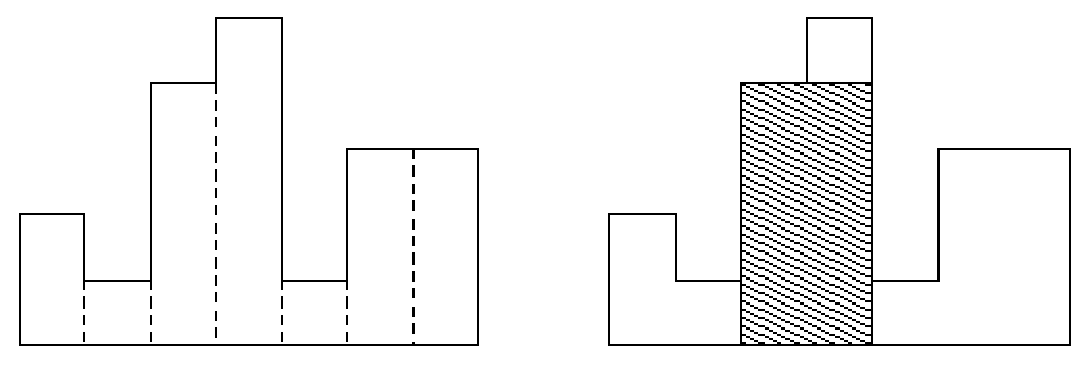
\includegraphics[width=10cm]{image.eps}
\end{center}

Usually, histograms are used to represent discrete distributions, e.g., the frequencies of characters in texts. Note that the order of the rectangles, i.e., their heights, is important. Calculate the area of the largest rectangle in a histogram that is aligned at the common base line, too. The figure on the right shows the largest aligned rectangle for the depicted histogram.

% Input format
The input contains several test cases. Each test case describes a histogram and starts with an integer $n$, denoting the number of rectangles it is composed of. You may assume that $1 \leq n \leq 100000$. Then follow $n$ integers $h_1, \ldots, h_n$, where $0 \leq h_i \leq 10^9$. These numbers denote the heights of the rectangles of the histogram in left-to-right order. The width of each rectangle is $1$. A zero follows the input for the last test case.

% Output format
For each test case output on a single line the area of the largest rectangle in the specified histogram. Remember that this rectangle must be aligned at the common base line.